
%(BEGIN_QUESTION)
% Copyright 2008, Tony R. Kuphaldt, released under the Creative Commons Attribution License (v 1.0)
% This means you may do almost anything with this work of mine, so long as you give me proper credit

The equation for determine volumetric flow rate ($Q$) of a liquid with a certain specific gravity ($G_f$) through a control valve given the upstream and downstream liquid pressures ($P_1$ and $P_2$, respectively) is as follows:

$$\includegraphics[width=15.5cm]{i03297x01.eps}$$

$$Q = C_v \sqrt{{P_1 - P_2} \over G_f}$$

The variable $C_v$ is called the {\it flow coefficient} of the control valve, and it varies from zero at full-closed to a certain maximum value (depending on valve size and type) at wide-open.

\vskip 30pt

Manipulate this equation to solve for downstream pressure ($P_2$) in terms of the other variables.  Be sure to show all your work!

\vskip 50pt

$P_2 =$

\vfil 

\underbar{file i03297}
\eject
%(END_QUESTION)





%(BEGIN_ANSWER)

This is a graded question -- no answers or hints given!

%(END_ANSWER)





%(BEGIN_NOTES)

$$Q = C_v \sqrt{{P_1 - P_2} \over G_f}$$

$${Q \over C_v} = \sqrt{{P_1 - P_2} \over G_f}$$

$$\left({Q \over C_v}\right)^2 = {{P_1 - P_2} \over G_f}$$

$$G_f \left({Q \over C_v}\right)^2 = P_1 - P_2$$

$$P_2 = P_1 - G_f \left(Q \over C_v \right)^2$$

%INDEX% Mathematics review: manipulating literal equations

%(END_NOTES)


